\chapter{Screenshots af SailingClubManager}\label{bilag:scm}

Dette bilag har til formål at underbygge afsnittet "\nameref{chap:teknologi-analyse}  (\ref{chap:teknologi-analyse})". Dette er et system, til administration af både, som vi har fået tilladelse til at prøve af skaberen. Siden hedder SailingClubManager, og er placeret på url'en \href{http://abs.boxstuff.net}{\textit{http://abs.boxstuff.net}}, "abs"\ da vores klub derunder hedder "Aalborg Boat Squad". Det er også muligt at anvende denne service til at lave sin egen hjemmeside til offentligheden, et eksempel på dette er: \href{http://www.thamessailingclub.co.uk/}{\textit{Thames Sailing Club}}.

\begin{figure}
	Siden /boats indholder de både, som er tilføjet af brugeren. \newline
	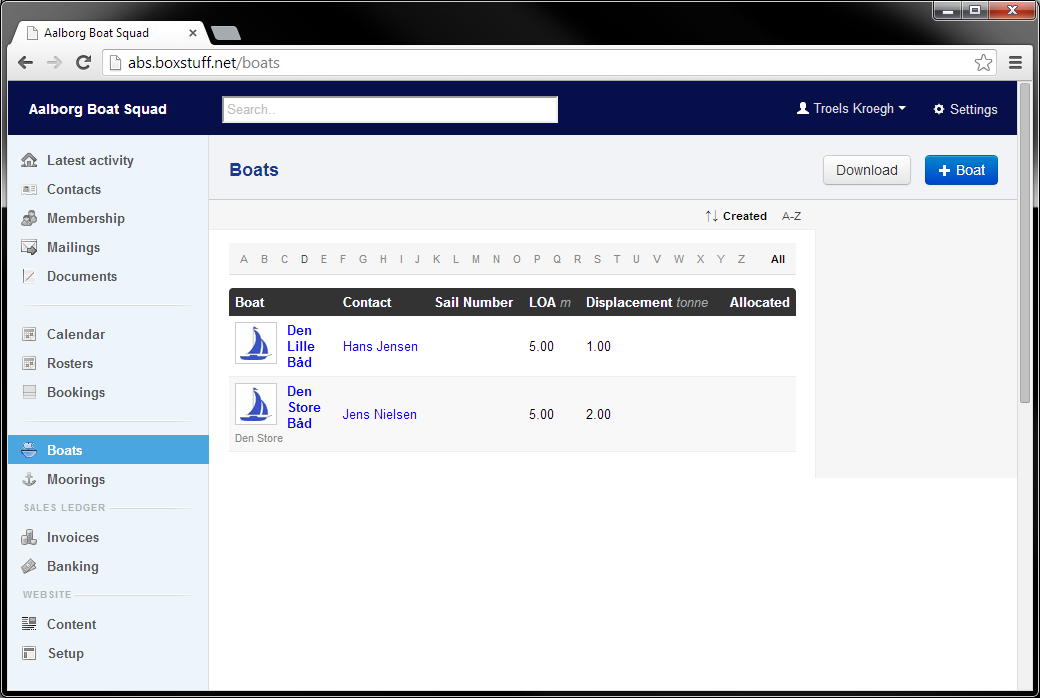
\includegraphics[scale=0.5]{images/teknologi/_Boats}
\end{figure}

\begin{figure}
	Personer som er en del af systemet, er en kontakt. De findes under /contacts.\newline
	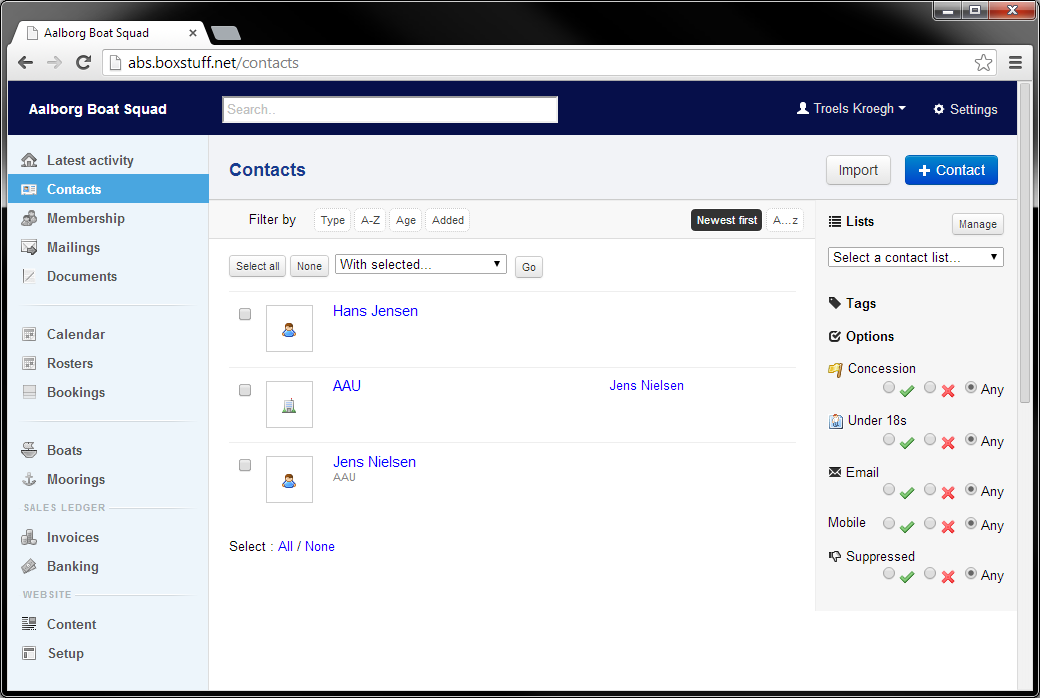
\includegraphics[scale=0.5]{images/teknologi/_Contacts}
\end{figure}

\begin{figure}
	Det er muligt at tilføje nye medlemmer, herunder hvilke type medlem de er. Disse typer er også muligt selv at lave i undermenuen Membership under /memberships/new.\newline
	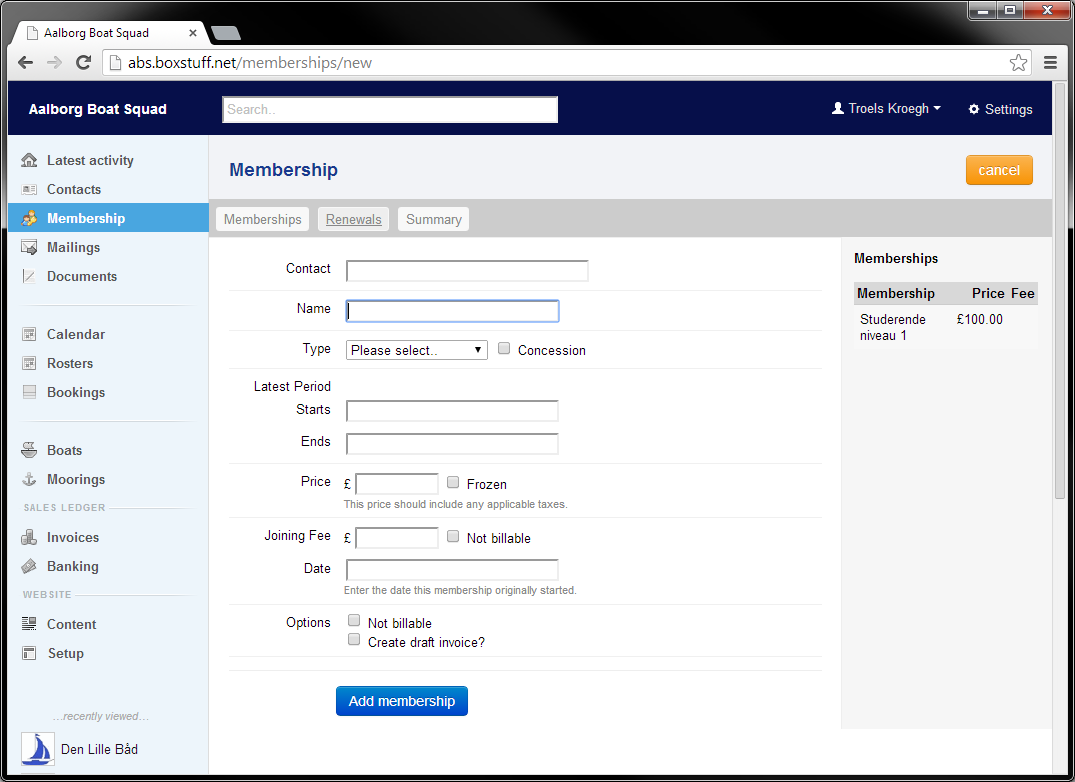
\includegraphics[scale=0.5]{images/teknologi/_AddMember}
\end{figure}

\begin{figure}
	Der findes en kalender med aktiviteter, som administratorer kan tilføje. Under /events.\newline
	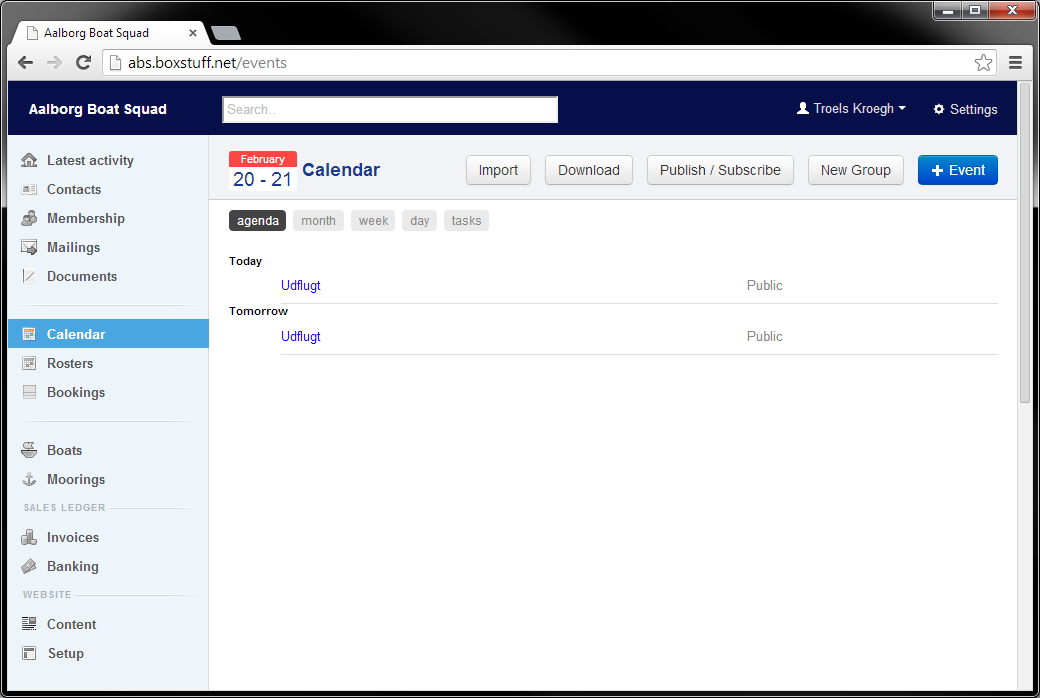
\includegraphics[scale=0.5]{images/teknologi/_Calendar}
\end{figure}

\begin{figure}
	Det er muligt for brugere at booke bådene, her har Hans Jensen booket en båd både den 20-02-2014 og den 26-02-2014. Dette findes under /booking/bookings.\newline
	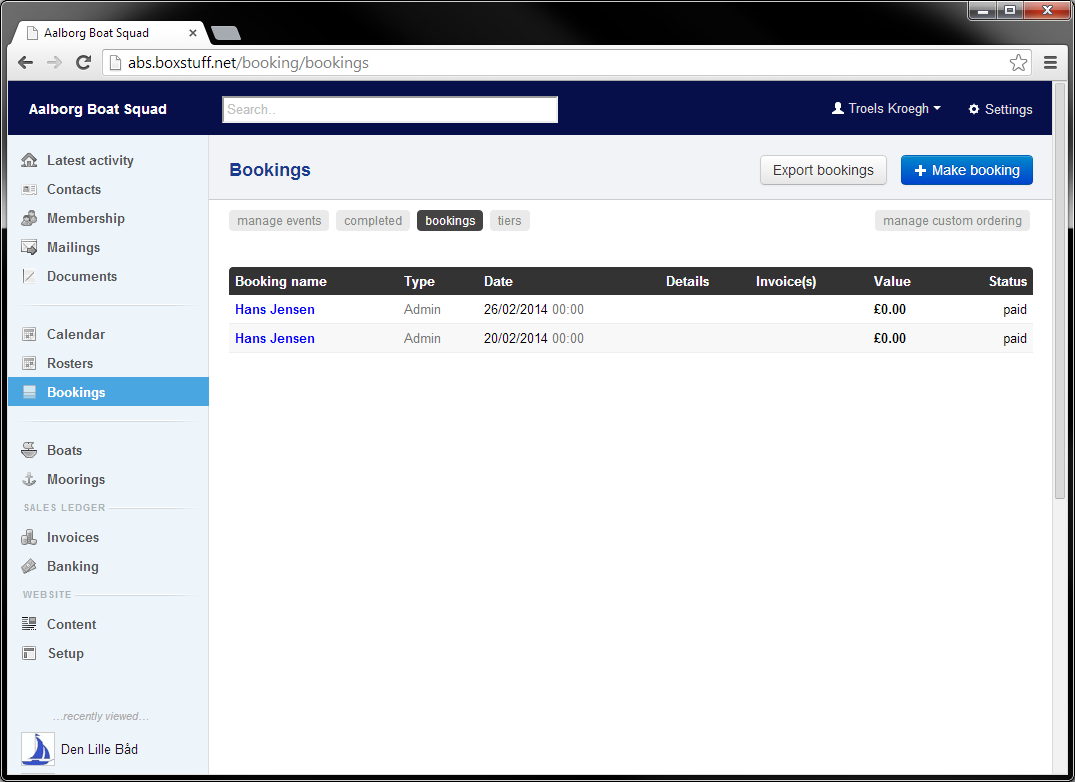
\includegraphics[scale=0.5]{images/teknologi/_Bookings}
\end{figure}

\begin{figure}
	Det er muligt at udskrive regninger baseret på brugeres udlån og kontingent. Under /invoices.\newline
	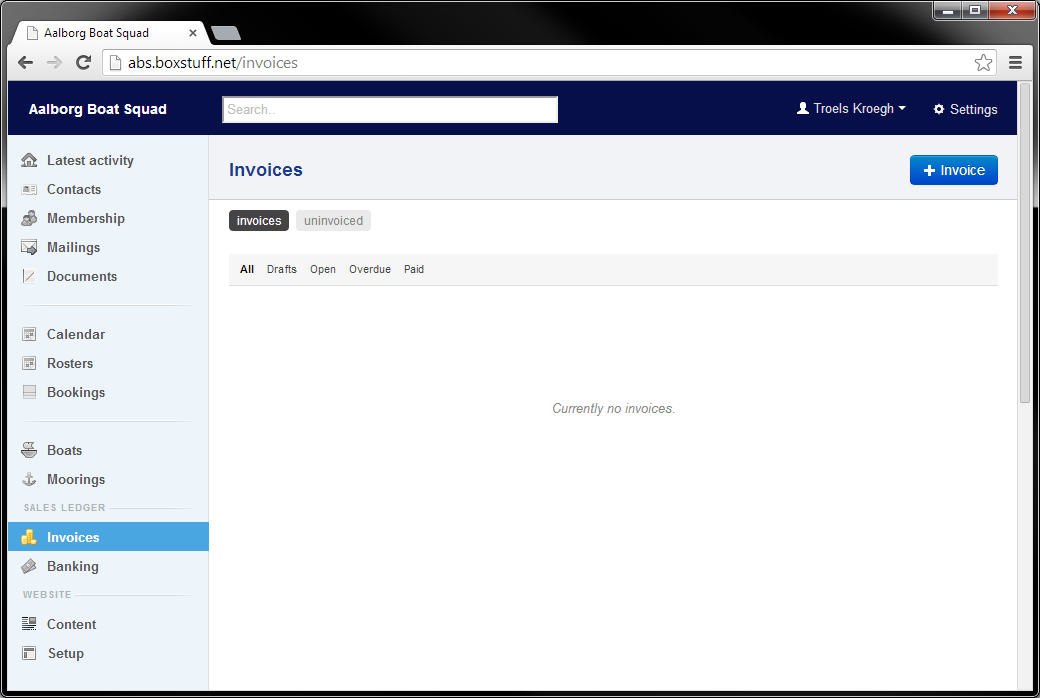
\includegraphics[scale=0.5]{images/teknologi/_Invoices}
\end{figure}

\chapter{Interview}\label{interview}
P- Peter Hinrup
D- Dorthe
K- Kasper
M- Mikkel
M2- Martin

P(00.00): der er 4 havne i aalborg hvor kommunen ejer havnen, hvor klubberne lejer havnen gratis imod at de selv vedligeholder den. Det er typisk en bådklub pr havn, ud over det bliver havnene nogle gange benyttet af andre mindre klubber så som kajakhavne eller søspejdere.

P(02.19): Der er 4 store havne i Aalborg, den her, Skudehavn, Marinafjordparken (aalborg sejlklub) og Nørresundby. De er ejet af Aalborg kommune imod at klubberne selv står for vedligeholdesen.

P(03.35): Vi er en forening med medlemmer som er medlemmer fordi de ejer en båd, hvorimod i Nibe kan man leje en plads, trods man ikke er medlem. I VB kan man ikke have en bådplads unden at være medlem.

P+D(05.00) viser gruppen en brochure med et kort over havnen.

P(06.25) Til sammen har VB og SL omkring 450 bådpladser, og i VB har de omkring 380 medlemmer og SL har omkring 150 medlemmer. I VB er det et familie medlemsskab, hvilket vil sige 1 båd = 1 medlem. 

D(07.31) Vores medlemskaber (SL) 	er pr hovede samt aktive og passive medlemmer.

P(08.00) Et medlem kan kun have en båd, dog i praksis ses det igennem fingrene, fordi det henner at et medlem køber en båd, også skal de have den gamle solgt. Det løses ved at et andet familiemedlem køber et edlemsskab

P(09.20) Dog sker det modsatte hvor der er flere ejere på en båd. Det er ofte unge mennesker der slår sig sammen omkring båden, men de skal alle være medlemmer, hvilket der ikke bliver tjekket op på.

D(11.40) SL og VB deler vandpladsen og betaler hver for sig leje til ANF. SL's medlemmer afregner pr kvadratmeter båd, hvorimod i VB, hvor de afregner pr pladskvadratmeter. Alle både beholder eller får nye pladser til foråret. Men man kan ikke købe en permanetplads, dog er der ballade hvis de flytter en båd der har ligget det samme sted i 20 år (Joke).

P(13.55) Pladser bliver også tildelt udfra forholdene på pladsen, f.eks. hvor dybt der er, men primært længde*bredde. Det er svært at få til at gå op i en højere enhed siden der er så mange inputs og interessanter man skal tage højde for.

P(14.49) hvert forår og januar måned går VB ud til alle medlemmer hvor de sender den information de har omkring deres medlemmer til dem, for at få opdateret den information der står i systemet. Derudover skal de også svare på deres ønsker til bådplads til sommer.	

D(16.00) Vi har kun sejlbåde i forhold til VB som har alle slags både

M2(16.35) "Hvad gør i med bådene fra medlemmer der er blevet smidt ud?"
P: Vi meddeler dem at de skal fjerne deres båd, og inden for en rimelig tidsrammer vil båden blive flyttet eller solgt

P(19.16) medlemmerne har numre, ældst har lavest nummer og vice versa. Dem med det mindste nummer har første ret på alt og det er besverligt for administrationen

P(20.00) Peter viser os regnearket med alt informationen "Ønskelisten"

P(22.00) VB er størrere end SL, men har også størrere fluktuering i blandt deres medlemmer. Dog afhængig af hvornår de startede nummersystemet

P(23.26) Peter viser os pladserne på "Ønskelisten" og forklare nummer systemet. Nummer ex. XXYY, XX= bro nummer YY plads på broen

P(24.40) Efter allokeringen af pladser, udsendes der regnigner hvor nogle medler fra og dernest sendes der rykkere hvor flere melder fra.

P(27.40) Der er en masse personlige, menneskelige og interesser der ikke fremgår af listen når der skal planlægges. Det er vigtigt for nogle mennesker hvor de ligger, det er afgørende.

P(31.56) VB har forskellige pladser, herunder Pælepladser, som er en fast bro, med en pæl man kan binde sin båd fast i både pælen og broen. Det er dyrt at fjerne pælepladser på grund af omkostninger. Anholts bruger Bøjer.

P(35.10) Peter viser os en Flydebro og den er praktisk fordi den aldrig oversvømmer, og pladserne er pratiske især hvis de er Y-bomme hvor man kan ændre på pladsens størrelse.

P: Men det så selvfølgelig umiddelbart smartere ud end dette her. Fordi det er moderne. F.eks. kunne man få det grafisk op. Dine både altså, Man tegnede simpelthen sin havn ind på skærmen. Og hvor vi kan få bådpladserne op her, så kan vi så se hvad for nogle der er ledige, og hvad for nogle som er optaget, og hvem der har en plads. og det er meget meget fint, og det var grafisk. Man kan selv tegne broerne, og så er der alle pladserne, hvor de røde er optaget og de grønne er ledige. Og så kunne man så flytte rundt med en kurser, und so weiter.

D: Det ligner så det de lavede til Marine booking?

P: Jo, du kan så køre booking oveni.

D: Ja, for du kan vidst booke en plads online i nogle havne, og så skal de jo vide hvor de sender båden hen, når de kommer ind af havnemunden(?).

P: Ja, det er jo en anden ting som vi ikke har snakket om. Det er jo gæster. For en ting er at man har en bådplads, du har en hjemmehavn. Det adskiller sig jo meget fra f.eks. camping verdenen. Lang de fleste har en campingvogn derhjemme, og så kører de rundt hist og her. Vi har jo i meget højere grad et hjemsted, for du kan ikke have en 40 fods båd liggende hjemme i din indkørsel. Det er vildt besværligt, fordi sådan en vejer jo 12 tons. Så du har en havn, hvor du skal ligge, og hvis du skal ligge i en havn, så skal du være medlem af en klub. Det kan så være meget udemærket, fordi for mange er det en vigtigt del af det sociale liv, nogle de har ikke andet en den her klub, havde jeg nært sagt, end den her klub. Og de kommer og feste og bruger klub faciliteterne, og laver grill party, og sågar var der nogle som holdte nytår her i klubben.

D: Ja vi holdte da nytår henne i vores klub, nogle af os.

P: Ja ja, og det er super. En stor del af vores omgangskreds er også bådfolk, som vi har fundet sammen med. Men udover dette så sejler vi ud i den store verden. De fleste af os. Nogle meget nogle lidt og nogle aldrig, men det er meget forskelligt. Det er gæstesejling. Dette sker i alle havne. En stor del af vores indtægtsgrundlag er gæster. Vi har tusindvis af gæster om året. Nogle én dag, nogle mange dage. Det betaler de for.

D: vi ligger også strategisk godt her i limfjorden.

P: Alle der skal igennem; hollændere, tyskere nordmænd og mange flere. Det er en meget vigtigt del af vores indtægtsgrundlag. Det skal man også kunne styre. De kommer og så skal de betale. Der står sådan en automat herude, hvor de kan trække en billet som de sætter på en båd når de har betalt. Der er så facilitet, med bad mm. ligesom på en campingplads. Det bliver nogle steder mere og mere med at man kan booke en plads. Det tror vi aldrig at vi kommer tid at bruge i vores klub, fordi vi fylder havnen op. Men der står i vedtægterne, at når et medlem ikke bruger sin plads, kan klubben leje den ud. Vi har i Danmark et rødt/grønt system. På pladsen nede på broen er der et skildt, hvor grønt betyder ledigt. Så når man kommer ind i en havn kigger man efter grønne skilte og en plads der er stor nok til ens båd. Så lejer man den plads i en periode. Så står der en dato på skiltet, med hjemkomst dato.

Nogle havne dedikerer broer direkte til gæster. Især i sverige. Dette gør at halvdelen af havnen er tom og den anden halvdel er proppet. Sådan gør de i sverige. Men hvis man har den slags gæstebroer, så er det mere og mere normalt at lave online booking. Det har nogle regler og nogle gebyr.

5:32:

D: Grafisk er kun interessant for gæster

P: Ja, det er kun farvelade

Martin: Er der medlemmer i klubben, som ikke kender layoutet, som kunne få hjælp af noget grafisk?

P: tjoo, men der ligger luftphotos og pladsliste på vores hjemmeside, samt vores brochure.

P: Det vores system ikke kan klare, er når det bliver mere advanceret adminstration. Det kræver at man både kan være EDB-mand, og økonomi man, og det tager en masse tid. Alle klubber uden undtagelse døjer med at finde folk der har evner og interesse. Min forgænger holdte et halvt år.

D: Jeg aner ikke noget omkring excel ark, og skal forsøge at bruge det nuværende.

P: Det er meget forskelligt, og det er frivillige i forengninger.

D: jeg er heldigvis kun afløser.

P: Det er et stigende problem, og flere og flere betaler sig fra det. Aalborg Sejlklub har en bogholder de lønner. Vi vil gerne slå os sammen i vores havn, og så lave en over-paraply. Det vil være ét system, som skal kunne holde styr på to klubber. Nogle ting er fælles, andre ting er seperate. f.eks. priser på vandpladser. Vi er en momsregisteret virksomhed, med en millionomsætning. Man ser i stigende grad, sammenslåning af administration på tværs af klubber der deler samme havn. Hvis vi nu f.eks. for et nyt medlem, og ikke har plads til ham, er det fjollet at vi ikke kan ligge ham på den plads lige ved siden af, som tilhører Sejlklubben limfjorden. Sådan kan vi ikke gøre nu.

10:19:

P: gæstesejlere kan ligge overalt, og det kunne være rart hvis vi kunne optimere noget der. Og når i snakker IT, så skal systemet kunne håndtere 2 havne delt på kryds og tværs imellem to klubber. Og det har vi ikke fundet noget system der kan.

P: Det er dyrt at få lavet ting til systemet.

D: Men man bruger også meget tid, som kasser.

P: Og hvis man så bruger tid på at lave hjemmeside og alt sådan noget, det kræver også tid. Det kræver også nogle evner.

D: Jeg administrerer vores fane på hjemmesiden.

P: Hvis vi skal have en ny bro koster det 1 million, 2 hvis det skal være med y-bom. At fjerne den gamle koster en halv, pga. miljøregler. Vi skal overholde nogle regler, hvis vi skal have tilskud fra kommunen.

P: For mange er en båd, den største investering i deres liv. Min båd koster mere end vores ejerlejlighed på havnefronten. Så det betyder noget. Nogle bor i båden, og har adresse her, med postkasser. Nogle klubber tillader ikke det her, men vi kan godt lide at der er folk i havnen.

D: nogle bruger båden som kolonihavehus, og sejler aldrig ud.

P: Vi har 2 ældre damer, hvor deres mænd er døde, og de er her næsten altid, men de sejler næsten ikke.


D: Efter vi har fået betaling til el, er det blevet nemmere at holde styr på. Vi fik installeret målere, så el bliver købt nu. Vi har også en fuldtlønnet havnefodge.

Kasper: Kommer han udefra?

P: Ja, han kommer udefra. Han må slet ikke have båd. Han arbejde 12-14 timer om dagen, om sommeren, og så holder han fri om vinteren. Det er lørdag, søndag, påske og pinse. Lidt som campingfatter på en camping plads. Det er lidt forberedelse før sæson. Havnefodgen er bl.a. service organ, og kan hjælpe til med informationer til turister, og f.eks. motorhjælp.

17:00:

D: Hvis vi har været ude og sejle, og kommer hjem en dag før planlagt, så ringer vi til Per (fogeden), og ber ham om at vende den rød/grønne plade. Hvis der så ligger nogle på pladsen, informerer han dem om at de skal finde en anden plads.

P: Dette sker hele tiden. og det er træls, men det er vilkårne, når man vil være fleksible. Fogeden står også for generel vedligeholdelse, som f.eks. maling og ukrudtfjernelse.


Kasper: Hvordan er fordeling af gæsterindtjeningerne?

P: engang var det efter pladser, men nu kører det efter nogle fordelingstal. I hovedhavnen for VB 60 \% og SL 40\%. I den anden havn har VB 100\% pga. suverænt flest pladser. Omkostninger på landpladser og andre faciliteter, bliver også delt. VB har ansat havnefoged, og skriver timesedler med fællesting. Denne løsning virker kun sålænge vi er gode venner.


P: historisk set, har der været lidt krig imellem klubberne. Efter den nye havn er der ikke så meget pladsmangel, men så er der nogle andre ting.


P: Frihavn er i bund og grund en bytning af pladser imellem klubber.


D: lysten til frihavnsordningen ligger bl.a. i en historisk holdning. Det bliver bestemt på generalforsamlinger.


P: I automaten kan man gøre 2 ting. Fylde penge på sit chipkort, eller leje en plads. Hvis man vil leje en plads skal man oplyse størrelsen på sin båd. der er 3 størrelses intervaller, samt et frihavns interval. Via en farvekode kan fogeden se hvor lang tid de har holdt der. hidtil har det været den samme pris hvorvidt man betaler havnefogeden eller i automaten, men det vil vi gerne have lavet om på, sådan at dem der betaler via automaten.


Kasper: er der udlejning af både?

P: Nej. Men der er visse firmaer som har både af representative årsager, men det vurderer vi ikke til at være "kommericelt"


Kasper: Hvordan er det med undervisning?

P: Vi har ikke noget undervisning.

D: Vi har lidt specifikt til sejlsskibe.

P: Nogle af skibene kræver beviser, rent lovgivningsmæssigt. 

Martin: Når der kommer nye medlemmer, tjekker i så om de har beviserne?

P: Det er et krav, men vi følger ikke rigtigt op på det.

D: Sejlbåde kræver ikke beviser.

P: vi kræver en ansvarsforsikring, ikke casco, og vi har en mulighed for en fælles forsikring.

D: Det har vi ikke, det er folks ejet problem.

P: Halvdelen af vores medlemmer har tilmeldt sig den kollektive. Men vi kan ikke holde styr på vores gæster.

Kasper: Ved i om der er nogle i ANF som udlejer både.

P \& D: ikke hvad vi ved af.

P: Nogle klubber tillader at man kan udeleje private både fra en klubhavn, men jeg har ikke hørt om en klub der udlejer.

33:00:


Martin: Kan jeres system klare udervisning?

P: Vi har slet ikke undervisning, men Aalborg Sejlklub har undervisning, og der er en uskreven aftale om at de ordner det for sejlklubberne i Aalborg. Der er ikke nok til at understøtte flere sejlhold.


Kasper: Hvor lang tid bruges der på administration?

P: Min kone siger 700 timer på et år på Vestre Baadelaug.


Peter: Det er svært at få besat bestyrelsesmedlemmer. Hos os skal man ikke betale kontingent når man sidder i bestyrelsen - en lille symbolsk betaling. Lovgivningen giver nogle muligheder i form af dækkende betalinger som f.eks. kørsel og telefon. Det kan ikke passe at det skal koste penge at være frivillig, så derfor udlignes udgifterne via specificerede takster.

Kasper: Så det er lysten der er drivkraften? Peter: Ja, hvis lysten ikke er der, skal man ikke gøre det.

Kasper: Omkring forsikringer. Peter: Vi har forsikret bestyrelsen, så hvis f.eks. kranen fejler og skader en person. Da vi har folk ansat, har vi også forsikring der. Også ved frivilligt arbejde i weekender hvor folk kan blive skadet osv. osv.

Kasper: Bare lige for at ridse op, så har i en stor turnaround af medlemmer, korrekt? Peter: Ja, for de (SL) har valgt kun at have sejlbåde, hvor vi (VB) er for flere bådtyper. Det gør at flere aldersgrupper er medlem i VB. I SL er medlemmerne ældre. Der er også forskel i filosofier i klubberne. I VB vægtes det sociale aspekt meget højt. Der er sejlture, fester osv. Mange andre klubber gør stort set ikke sådan noget.

Kasper: Lidt omkring ANF. Samarbejdet mellem klubberne - hvordan er det? Peter: Nogle af de penge fra kontingentbetalinger ryger hen til ANF. Disse penge går til vedligeholdelsen af alle havne tilknyttet ANF. ANF har en aftale med kommunen, den såkaldet brugsaftale. Aalborg kommune har udlejet havnearealerne til ANF som så distribuerer dette til klubberne. Det kører rigtig godt, og har gjort sådan i over 20 år.

Kasper: Deler alle klubber samme holdning? Du nævnte noget klubfjenskab mellem AS. Peter: Klubfjenskab hænger sammen med nogen af de nye folk de har fået. For 30 år siden var der trængsel om pladsen. Kommunen blev overbevist om at bygge en ny havn - Marina Fjordparken.

P(50.00) Kommunen byggede den nye havn fordi de 5 klubber skændtes omkring havne
pladserne. De gik til kommunen som bygge den nye havn og de tilbød at flytte 
derud hvis de selv stod for vedligeholdelse. Aalborg Sejlklub som var størst og ældst
flyttede til havnen. Betingelsen var også at de selv skulle betale for rennoveringen
af de gamle havne.

P(51.30) ANF bruger mange af pengene til rennovation men Aalborg Sejlklub 
udviser ikke interesse for at være med i det fællesskab, trods der mangler
8 millioner kroner i renovationer for at komme på samme niveau som
Aalborg Sejlklub (Der er strid omkring dette).

P(53.10) ANF er unikt for aalborg siden det plejere at være individuelle havne
som har hver deres klub som ikke samarbejder med de nærliggende, ifølge Peter

P(54.00) Klap tilladelse på ANF niveau, gør at de må depositere det jord de graver ud,
hvis da ikke det er forurenet, i en nærliggende havn, som har plads til det.
Dette skulle eftersigende ændre prisen fra 400.- pr kubikmeter til 40.- pr kubikmeter

Kasper: Indførelse af det nye IT-system, hvornår var det?
Peter: Jeg mener det var i 05'. Jeg blev kasserer i 07. Siden det har vi fået lavet en hel del tilføjelser. F.eks. det der mail-fletning, mail-afsending. Vi fik også mail adresser på alle medlemmer. Før det, sendte vi breve ud til alle medlemmer.

Martin: Ved du hvad i gjorde før 05'?
Peter: Ja, der havde man et eller andet ældgammelt system. Også IT-baseret. Giro-kort blev sendt ud til medlemmerne, og breve blev sendt flere gange om året.

Kasper: Hvordan er IT-systemerne i ANF?
Peter: Det er meget forskelligt. Sejlklubben Limfjorden kører med Excel, og er derved meget bagud. Vi (Vestre bådlaug) snakkede om at gå sammen med SL i stedet for. Problemet i SL er at kasseren ofte er ude at rejse, hvorfor en midlertidig kasser benyttes. Det er svært at finde nye kasserer. Min forgænger holdt kun et halvt år; det er et fuldtidsjob. Det er tidskrævende og der er masser af deadlines, f.eks. NETS til betalingsservice. Man skal være temmelig skrap til f.eks. NEM-ID, hjemmesider. Det hører også sammen med at det er en relativ stor forening med en relativ stor omsætning.

Kasper: Registreringer af diverse ting; har i nogle registreringssystemer som ikke er inkluderet i diverse IT-systemer.
Peter: Ja, udover navision har vi et system til håndtering af nøglekort. Alle medlemmer skal have mindst 1 kort med en chip. Dette er deres medlemskort. Det virker til døre, bad osv.

Kasper: Ville det være smart hvis dette system blev inkluderet i medlemssystemet?
Peter: Ja, det ville være smart at lægge systemerne sammen, men det er meget bøvlet, fordi nøglesystemet er meget integreret med boksen der holder styr på nøglerne.Her er der redundans. Dvs. her er der også et medlemskartotek. Blokering af kort osv. 

Kasper: Hvis disse problemer ikke havde været til stede, havde i så valgt at sammenlægge systemerne?
Peter: Ja, det er klart, redundans information er fandens værk.

Martin: Hvis man kunne optimere noget af den tid der bruges på indtastning af medlemmer, f.eks. ved at de selv kunne indtaste noget. Er der noget du (Peter) bruger meget lang tid på?
Peter: Når vi skal have informationer fra medlemmer, kommer de typisk ind fra mails. Så skal de skannes, og så skal man se om der er sket rettelser i forhold til gamle information. Hvis dette er tilfældet, skal dette bogføres i systemet. Jeg ville aldre få medlemmerne til selv at indtaste dette. Skemaerne fra medlemmerne skal arkiveres. De bliver smidt ind i en mappe på computeren. Man skal også se om der er ønsker til bådpladser. Der ligger en helvedes masse arbejde. Nogle pladser skal flyttes. Det er et stort arbejde.

Minut 10

Kasper: Hvis brugerne kunne indberette i nogle formularer, som systemet kunne bogføre nemmere..
Peter: Nej.. Et andet aspekt er kontingentbetalinger. Man kan fra NETS hver dag downloade hvilke betalinger der er foretaget. Dette kan man automatiske opdatere, men det har jeg valgt fra. Så har jeg bedre styr på hvem der har betalt. Det kan man dog sagtens lave automatisk. Man skal dog holde styr på special cases. Til gengæld hvis der havde været 4000+ medlemmer, havde det været relevant.



Peter: Hvis et medlem får en større båd, skal dette medlem selvfølgelig også have en større plads. Nye medlemmer der kommer ind, skal betale kontingent. Det sker via indbetalingskort, uden brug af NETS. Der er altså ikke meget tid at hente ved indtastning.

Kasper: Er der nogle udefrakommende lovmæssige krav til hvad der skal registreres?
Peter: Der er det skattemæssige, vi skal ikke betale skat. Til gengæld skal vi registrere MOMS, digital postkasse, NEM-ID. Registreing til forskudsberetning, registrering til Aalborg kommune. Dette giver et tilskud på 200.000 kr. om året. Dette er i øvrigt alt for meget, efter min mening. Derudover kommer medlemskab af DSU osv. Der er ingen der siger at man skal bogføre med et IT-system. I princippet kunne man godt have pengene i en cigarkasse. Registreringer er altså ikke det værste.

Kasper: Hvem er i kontakt med IT-systemet?
Peter: Det er mig. Der er flere der bruger det, men det er mig der styrer det. Jeg sørger for backup og administrationen af systemet.

Martin: Hvem bruger det ellers?
Peter: I teorien burde alle bruge det, men i praksis bruger sekretæren det, og vores aktivitetsleder. Derudover fartøjsinspektøren. Næstformanden og formanden bruger det ikke. Det varierer på hvem der sidder i bestyrelsen. Vi bruger Dropbox i stor stil til deling af dokumenter. Jeg kunne godt ønske mig at nogen var mere med på beatet, teknologisk set. Et problem var at der ikke blev lavet backup i et helt år. Det kunne have gået meget galt. Det er altså vigtigt at der er en IT-administrator.

Kasper: Omkring platforme, du nævner at du har adgang fra klubhuset og hjemmefra. Er der andre steder i har adgang, f.eks. telefoner, iPad's.
Peter: Det kan man lave, men det har vi ikke.

Kasper: Er der interesse i et system med fjernadgangsmuligheder? Nu nævner du at der er en del unge. Kunne det være smart hvis de kunne se oplysninger omkring deres båd f.eks.?
Peter: Nej..
Martin: Der er heller ikke noget medlemmer skal indmelde løbende?
Peter: Nej ikke løbende, kun ændringer som f.eks. nyt telefonnummer eller email. Ellers 1 gang i året ved plads tildeling og opdatering af informationer. Hvis medlemmerne betaler de 2 regninger om året, og de ikke flytter, skal der ikke registreres nogle informationer.

Kasper: Hvilke udgifter har i til det nuværende IT-system?
Peter: Det sku' billigt. Altså vi har jo super internetforbindelse, den koster selvfølgelig lidt. Derudover den nøgleautomat. Derudover er der software-licens til Navision, office har vi købt. Navision licensen koster omkring 5000 kr/året. Så er der noget omkring hjemmeside hosting, men det er småtingsafdelingen. Så er der diverse nye printere osv.

Lige omkring minut 20

Kasper: Kan du opsummere nogle af de punkter, hvor man kunne ønske sig forbedringer?
Peter: Ved vores nuværende system, kan man ikke lave en regning og sende den via mail. Men det skal bare laves, der er ingen problemer i det. Det kan være vi alligevel skal have et nyt system. Et andet godt system til bogføring er e-conomic.dk. Det er helt vildt godt - cloud baseret og det hele. Det er dog ikke nødvendigt at det er cloudbaseret for vores behov. Jeg har alligevel remote-desktop adgang.

Martin: Havnefogeden, ved du hvordan han holder øje med hvorvidt folk er ude eller hjemme?
Peter: Han er der stort set i døgndrift i sæsonen og han kender efterhånden gud og hver mand. Der er ikke noget formelt system som sådan.
Martin: Det var måske en mulighed. Du talte om at andre havne har et system, hvor gæster kan se om folk er ude og/eller hvornår de kommer hjem.
Peter: Nej, ikke nødvendigvis. Det er fordi de har dedikeret gæstepladser, så de har booking af gæstepladser. Det kan vi ikke gøre, fordi vi ikke har dedikerede gæstepladser. I skal huske på at vi i sejlbranchen er meget afhængige af vejret. F.eks. regner man med at man skal sejle hjem søndag, men man finder ud af at der er stormvarsel. Man ligger nu på Anholt. Det gælder altså om at skynde sig hjem inden stormen kommer. Man laver altså ofte om i planen. Man kan altså ikke langtidsplanlægge. Vores system fungerere så ved at man kan melde havnefogeden hvornår man regner med at være hjemme igen. I tilfælde af at man skal før hjem, må man ringe til havnefogeden. Havnefogeden holder styr på alle disse informationer på sin egen måde ved en kuvert eller andet.

Martin: Det kan godt være det er fint for ham, men en ny havnefoged, vil have hjælp af en bedre organisation. Desuden vil gæster, hvis det var cloud-baseret kunne se hvor der var pladser.
Peter: Jo, men så skal dette system opdateres hele tiden når folk en plads er fri.Vi har 2 havne, over 400 havne. Om eftermiddagen kan der ske at der kommer op til 25 sejlbåde på en gang. Der er så kaos om at finde en plads. Gæsterne har mange præferencer i forhold til hvordan de vil ligge i forhold til vinden osv. osv. osv. Det er ikke som en campingplads, hvor man holder udenfor porten, og går ind til campingfatter og spørger om en plads. Så kigger han på kortet, og ser at en specifik plads er ledig. Andre steder kan man selv vælge mellem ledige pladser. Ved valg af plads, sætter campingfatter et kryds, og spørger om hvor lang tid man regner med at campere der. Når man tager hjem, går man ind til campingfatter og betaler. Så kan han registrere at pladsen er ledig. Det kan vi ikke gøre i sejlklubber. Nogen gange kommer de ind om natten.

Martin: Hvordan gør man med betaling når gæsterne ankommer?
Peter: Normalt skal gæsterne gå op til en automat, men ellers finder havnefogeden ud af at de er ankommet den næste morgen.

Peter: Om sommeren kan der være 100 gæster på en dag, og så kan man ikke styr det mere.
Martin: Du siger at de skal betale for pladsen i automaten. Kunne man ikke få gæsterne til at indtaste informationer ved pladskøb? 
Peter: Det kræver at de kender hvilken plads de holder på. Der er både hollændere, polakkere, svenskere osv. Alle mulige sprog, og derfor er registreringen for omfattende. Ofte er fejlagtig information værre end ingen information. Den store forskel på en sejlklub og en campingplads, er at vi ikke holder styr på hvem der kommer og går - det må vi ikke. Det er en offentlig havn. I tilfælde af nødstilfælde, skal man kunne komme ind i havnen.

Peter: Jeg kan ikke se hvordan man kan lave et smart system. Man er nødt til at indse at ikke alle folk er lige snue.